\setchapterpreamble[u]{\margintoc}
\chapter{Summary and Future Outlook}

\section{Summary of Results}
\label{sec:summary}

This work presented two oscillation measurements of atmospheric neutrinos using the DeepCore sub-array of the IceCube Neutrino Observatory. Both measurements were based on a newly developed data sample of \num{21914} well-reconstructed, track-like events

\subsection{Three-Flavor Oscillations}
\label{sec:summary-three-flavor}

The three-flavor oscillation measurement presented in \refch{measurement-three-flavor} was based on a newly devloped data sample of \num{21914} well-reconstructed, track-like events.

\subsection{Sterile neutrino search}
The second measurement presented in this work was the search for eV-scale sterile neutrinos. The search was performed under the "3+1" model, where the PNMS matrix is extended by an additional row and column to accomodate the mixing of a fourth neutrino mass eigenstate. The measurement used the same data sample as the three-flavor fit and the same likelihood function calculated in an identical binning. The major technical difference between the analyses was that the neutrino oscillation calculation for the sterile neutrino model was done using a customized version of the \textsc{nuSQuIDS} package. It allowed a computationally efficient way of calculating flavor transition probabilities in the presence of a heavy fourth mass eigenstate that produces a very fast oscillation pattern. The customizations that were developed specifically for this work were the addition of low-pass filters that can analytically produce oscillation probabilities where the contributions due to that heaviest mass eigenstate are averaged out. Another major technical development that separates the sterile neutrino analysis from the three-flavor fit is the introduction of a novel method of incorporating uncertainties in the detector response in a way that is fully decoupled from neutrino oscillation probabilities.

\subsubsection{Result}
The analysis constrained the $|U_{\mu4}|$ and $|U_{\tau4}|$ elements of the extended PNMS matrix to\todo{extract precise numbers}
\begin{equation}
    \begin{aligned}
        \abs{U_{\mu4}}^2 &< X \\
        \abs{U_{\tau4}}^2 &< Y \\
    \end{aligned}
\end{equation}
at 90\% C.L. while marginalizing over the CP violating phase $\delta_{24}$. This result is valid for both normal ordering and inverted ordering thanks to the approximate degeneracy between the mass ordering and the sign of $\cos(\delta_{24})$. The confidence limits were calculated using Wilks' theorem assuming two degrees of freedom. Spot-checks of the likelihood distributions showed that these limits err on the conservative side. More stringent limits could be obtained by correcting the critical values of the likelihood according to Feldman and Cousins\cite{Feldman_1998}, but the computational expense was deemed too high and the conservative limits sufficient for the purposes of this work. This result is a substantial improvement over the previous DeepCore result and provides the most stringent limit on $\abs{U_{\tau4}}^2$ to date. The constraint on $\abs{U_{\mu4}}^2$ is competitive with other experiments and has the potential to further increase the tension between appearance and disappearance datasets in global fits of the 3+1 sterile neutrino model described in \refsec{global-anomalies}.

\subsubsection{Opportunities for improvement}
A substantial increase in the sensitivity of the analysis could be achieved by using the table-based reconstruction method described in \cite{lowen-reco-paper}. This algorithm can provide an estimate for the energy and zenith angle for nearly all events passing the Level 5 event filter described in \refsec{data-processing} and has a much higher resolution than the reconstruction method used in this analysis, substantially increasing the statistical power of the analysis. The projected sensitivity that could be achieved with this method is shown in \reffig{retro-sensitivity}.\todo{Compare SANTA sensitivity} With the increased statistical power and resolution also comes a larger burden to accurately model the properties of the neutrino flux, particle interactions and detector properties. The work to bring data and simulation into agreement with the more powerful sample is still ongoing at the time of writing this thesis.
\begin{figure}
    \centering
    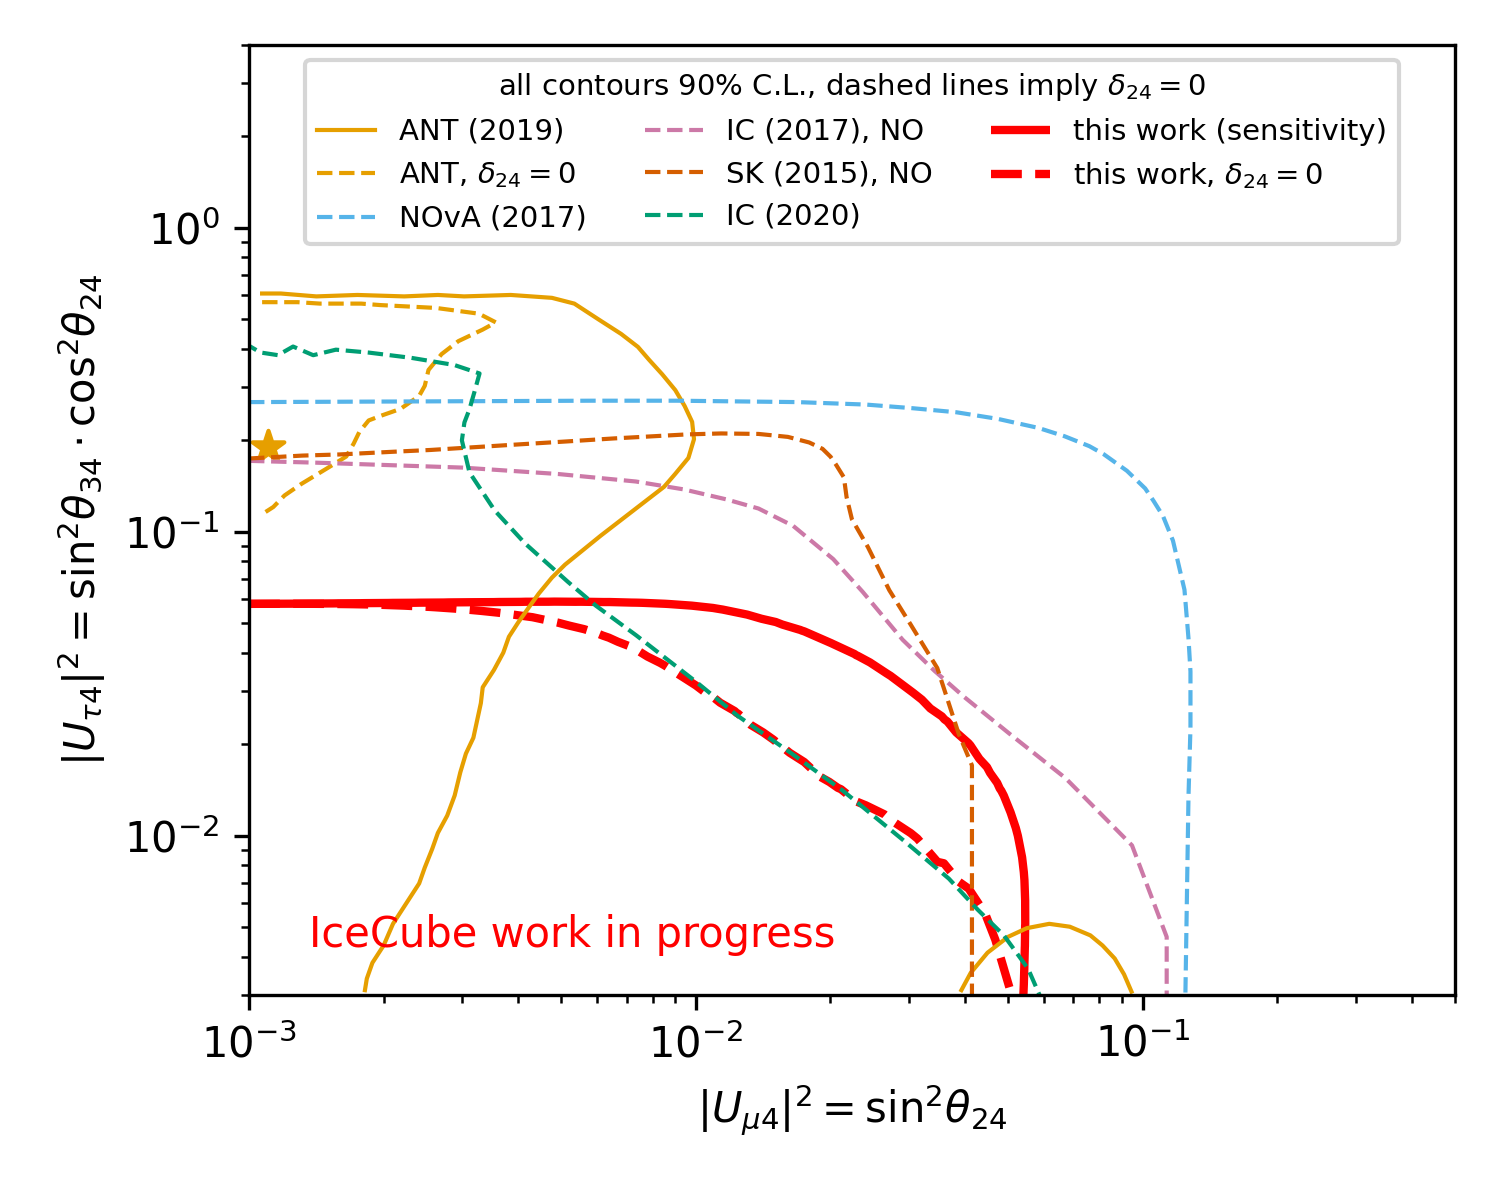
\includegraphics{figures/summary/Sterile_mixing_sensitivity_90pct_retro.png}
    \caption{Projected sensitivity of the sterile neutrino search when using the table-based reconstruction method.\label{fig:retro-sensitivity}}
\end{figure}

\chapter{Conclusion}

Since the experimental confirmation of the phenomenon of neutrino oscillations, they have
